\section{Results}\label{results}
Using some \textit{api} from Castalia Simulator some results like the total number of control packets exchanged, the total number of measurements packets, how many times a packets was retransmited among many others results can be obtained easily.

\subsection{Use case and simulation parameters}

Monitoring and Independent living for elder care is one of the use context of 11073 standard. The sensors and devices used for this use case is described in \cite{b3} is blood pressure, thermometer, glucose meter, pulse oximeter and basic ECG. In this work we used a hypothetical elderly patient who has cardiac problems, diabetes and hypertension and  after a major surgery needs to be monitored in his home.

The Fig.~\ref{fig:wbantopology} shows the topology setup used in our simulation. The hub node is placed at the right hip, one sensor node at the right and left wrist, one sensor node at the right and left ankle and one sensor on chest. The deployment of nodes is not the ideal, we just use this set to test our feature. The positions of nodes was maintained as they are in Castalia because real experimental measurements of path loss was made for every pair of nodes in \cite{b4}.

\begin{figure}[htbp]
\centerline{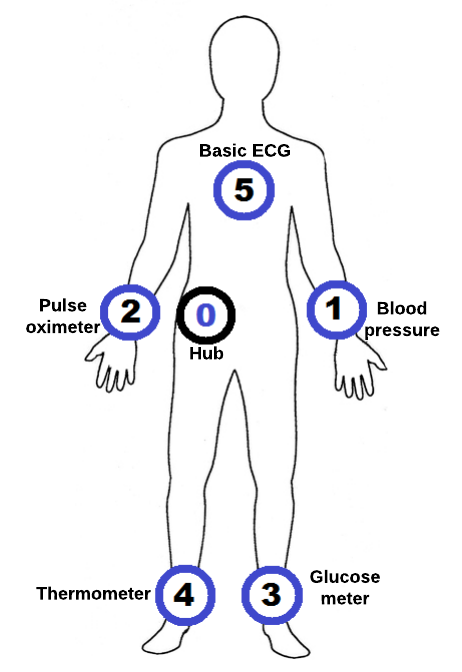
\includegraphics[scale=0.31]{figures/corpoSensoresNomes.png}}
\caption{The simulated network topology.}
\label{fig:wbantopology}
\end{figure}

In this paper we will simulate three scenario. The first scenario, called \textbf{unconfirmed mode} the agents will send measurement with no confirmation by the manager. The second, \textbf{retransmission mode} the agents expect an ACK from the manager and in case of an ACK not received the packets is just retransmitted. The third and last one, when an ACK is not received, the agent has to try a new assocition to finalize the transmission of the measurements packets. Table \ref{3modes} summarizes the three modes mentioned. The MAC layer used is the IEEE 802.15.6 with path loss map and temporal model for wireless channel supplied by Castalia and 1024 Kbps of physical data rate. The radio used meets with the IEEE 802.15.6 radio proposal \cite{b5} and $-15$dBm as transmission power.

\begin{table}[htbp]
\caption{The 3 modes supported by this work}
\begin{center}
\begin{tabular}{lllll}
\cline{2-4}
 & \multicolumn{1}{c}{\textbf{\begin{tabular}[c]{@{}c@{}}Unconfirmed\\ mode\end{tabular}}}                      & \multicolumn{1}{c}{\textbf{\begin{tabular}[c]{@{}c@{}}Retransmission\\ mode\end{tabular}}}                                      & \multicolumn{1}{c}{\textbf{\begin{tabular}[c]{@{}c@{}}Confirmed\\ mode\end{tabular}}}                                         &  \\ \cline{2-4}
 & \begin{tabular}[c]{@{}l@{}}The measurements \\ are transmitted\\ with no ACK from\\ the manager\end{tabular} & \begin{tabular}[c]{@{}l@{}}The measurements \\ are retransmitted\\ if an ACK is not\\ received from the\\  manager\end{tabular} & \begin{tabular}[c]{@{}l@{}}If an ACK is not\\ receied, try a\\ new association\\ to continue the \\ transmission\end{tabular} &  \\ \cline{2-4}
 &                                                                                                              &                                                                                                                                 &                                                                                                                               &  \\
 &                                                                                                              &                                                                                                                                 &                                                                                                                               & 
\end{tabular}
\label{3modes}
\end{center}
\end{table}

The configuration of the nodes is set as follow: the node 0 uses the \textit{Manager} application and is the hub. The blood pressure and the pulse oximeter transmit one measurement per second, totalizing 100 measurements to be sent in our simulation of 100 seconds. The thermometer convey one read every 2 seconds then 50 measurements should be sent. The glucose meter  transmit one measurement every twenty five seconds that is 4 measurement in 100 seconds. In this work we assume the basic ECG is a device that receives the signals of all electrodes deployed in the body and transmit these signals to the Manager. It will transmit 80 millivolts samples per 0.8 seconds what gives 125 measurements packets in 100 seconds of simulation.

\subsection{Statistical information of the proposed implementation}

All the results that will be presented is already implemented in the proposed application and everyone can feel free to customize it. The information results available in the application are the total control packets exchanged per node, the measurements packets received by the manager per node, the measurements packets sent by each node, and the total of associations made per agent. 

The first result discussed is the total of successfully measurements delivered to the manager. As described in \cite{b1}, when an agent is working on confirmed mode, it  should send a measurement packet and wait for the ACK during three seconds. This is so much time to wait in the absence of a transport layer. We can see in Fig.~\ref{fig:measurementreceivedpernode} how badly the confirmed and the retransmitted mode was because of this timeout. The unconfirmed mode delivered almost all the packets, even being a mode with no reliability.

\begin{figure}[htbp]
\centerline{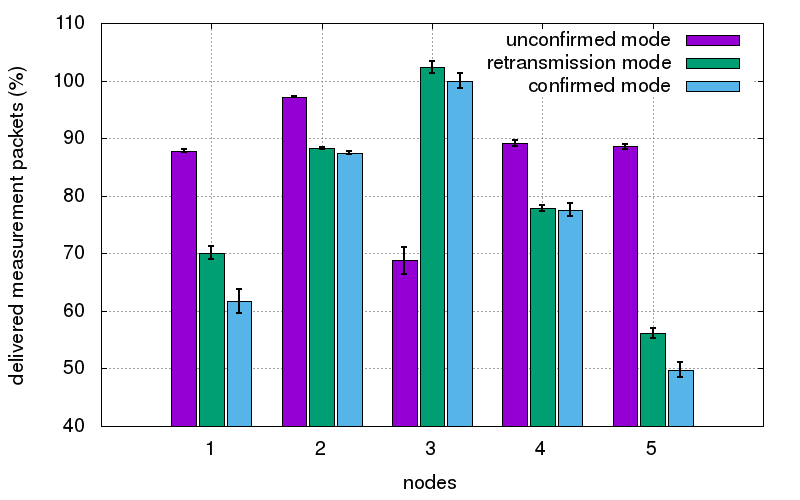
\includegraphics[scale=0.4]{figures/averagemeasurementpacketreceivedpernode.png}}
\caption{The average measurement packets successfully delivered per node}
\label{fig:measurementreceivedpernode}
\end{figure}

The control packets exchanged between a node and the manager is high when new associations has to be done in case of a non received ACK. The association process involves a maximum of four packets and two packets when the agent's attributes is previous know. Well, is depicted in Fig.~\ref{fig:controlpacketsexchanged} the total average of control packets exchanged between each node and the manager per mode of operation. Note that our retransmission mode implementation saves about $21.5\%$ of control packets when compared to confirmed mode. The unconfirmed mode as expected is the one that transmit less control packets.

\begin{figure}[htbp]
\centerline{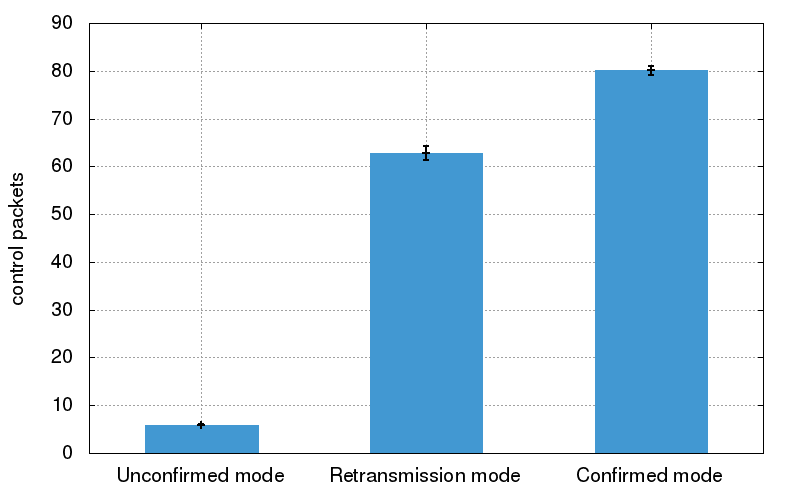
\includegraphics[scale=0.4]{figures/averagecontrolpacketsexchanged.png}}
\caption{The average control packets exchanged of all nodes in each mode}
\label{fig:controlpacketsexchanged}
\end{figure}

The number of associations made per node is extremely high with confirmed mode since it try always a new association after a packet is lost. The Fig.~\ref{fig:associationnumber} shows the average number of association that each node made in the three operation modes. As expected the confirmed mode has the highest average of association while the unconfirmed mode made just one association. The retransmission mode try a new association after have tried all the attempts to resend the packet or if receives an abort message form the manager, that's the reason for this mode have had a low average of association.   

\begin{figure}[htbp]
\centerline{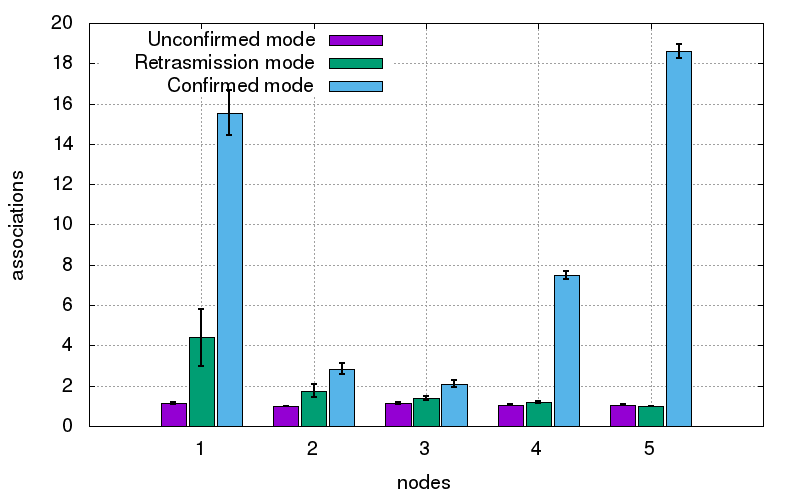
\includegraphics[scale=0.4]{figures/averagetotalassociationsmade.png}}
\caption{The average numbers of association made per node}
\label{fig:associationnumber}
\end{figure}